\chapter{Mathematical Formulation}
\label{cha:math-form}

This chapter presents the mathematical foundations underlying the solver
developed in this work. We begin with a detailed derivation of the Generalized
Minimal Residual (GMRES) method, including the construction of Krylov subspaces,
the Arnoldi orthogonalization process, the use of Givens rotations to solve the
resulting Hessenberg least-squares problem, as well as the preconditioning
technique and restarting strategies. We then describe iterative refinement in
the mixed-precision setting, highlighting the error correction model and the
distinct roles of factorization precision, working precision, and residual
precision. The chapter continues with a treatment of incomplete factorization
techniques, including incomplete LU with level-of-fill (\texttt{ILU(k)}) and the
fine-grained parallel ILU method.

\section{GMRES Method}
\label{sec:gmres-algorithm}

The Generalized Minimal Residual (GMRES) method, first proposed by
\textcite{saad_gmres_1986}, is a widely used iterative method for the numerical
solution of sparse, non-symmetric linear systems. As a member of the Krylov
subspace methods, GMRES approximates the solution by finding a vector within a
constructed Krylov subspace that minimizes the residual. This is achieved by
building an orthogonal basis for the Krylov subspace, commonly through the
Arnoldi process.

\subsection{Krylov Subspace Basis Construction}
\label{sec:kryl-subsp-basis}

Consider a nonsingular linear system of the form
\begin{equation}
  \label{eq:axb}
  \matr{A} \vec{x} = \vec{b}, \quad \matr{A} \in \mathbb{R}^{n \times n}, \vec{b} \in \mathbb{R}^n
\end{equation}
where \(\matr{A}\) is typically non-symmetric and sparse. Starting with an
initial guess \(\vec{x}_0\) and residual \(\vec{r}_0 = \vec{b} - \matr{A}
\vec{x}_0\), GMRES constructs the Krylov subspace
\begin{equation}
  \label{eq:krylov}
  \mathcal{K}_k(\matr{A}, \vec{r}_0) = \spann{\vec{r}_0, \matr{A}\vec{r}_0, \matr{A}^2\vec{r}_0, \dots, \matr{A}^{k - 1}\vec{r}_0},
\end{equation}
and seeks an approximate solution \(\vec{x}_k\) in the affine space \[\vec{x}_k
  \in \vec{x}_0 + \mathcal{K}_k(\matr{A}, \vec{r}_0).\] The approximation
\(\vec{x}_k\) is chosen to minimize the residual norm:
\begin{equation}
  \label{eq:argmin}
  \vec{x}_k = \argmin_{\vec{x} \in \vec{x}_0 + \mathcal{K}_k(\matr{A}, \vec{r}_0)} \norm{\vec{r}_0 - \matr{A} \vec{x}}_2.
\end{equation}

\subsection{Arnoldi Process}
\label{sec:arnoldi-process}

The vectors \(\vec{r}_0, \matr{A}\vec{r}_0, \matr{A}^2\vec{r}_0, \dots, \matr{A}^{k - 1}\vec{r}_0\) from
\eqref{eq:krylov} might be close to linearly dependent. So instead of this
basis, the Arnoldi iteration is used to extract an orthonormal one \(\vec{v}_1,
\vec{v}_2, \dots, \vec{v}_k\) for \(\mathcal{K}_k(\matr{A}, \vec{r}_0)\),
typically via the modified Gram-Schmidt (MGS) orthogonalization. The process
begins with a normalized basis vector \[\vec{v}_1 =
  \frac{\vec{r}_0}{\norm{\vec{r}_0}}_2.\] For each recurrence \(1 \le j \le k\),
a new vector \(\vec{w} = \matr{A} \vec{v}_j\) is orthogonalized onto the
subspace generated by \(\vec{v}_1, \vec{v}_2, \dots, \vec{v}_j\) via MGS:
\[h_{i,j} = \vec{v}_i\transpose \vec{w},\;\vec{w} \coloneq \vec{w} - \sum_{i = 1}^{j} h_{i,j}\vec{v}_i,\; h_{j+1,j} =
  \norm{\vec{w}}_2,\; \vec{v}_{j+1} = \frac{\vec{w}}{h_{j+1,j}},\] where
\(h_{i,j}\) are coefficients forming an upper Hessenberg matrix
\(\bar{\matr{H}}_k \in \mathbb{R}^{(k+1) \times k}\). In matrix form, the
process produces the Arnoldi decomposition:
\begin{equation}
  \label{eq:arnoldi}
  \matr{A}\matr{V}_k = \matr{V}_{k+1} \bar{\matr{H}}_k,
\end{equation}
where \(\matr{V}_{k} \in \mathbb{R}^{k \times n}\) has orthonormal column vectors
\(\vec{v}_1, \vec{v}_2, \dots, \vec{v}_k\).

\subsection{Least Squares Problem and Givens Rotations}
\label{sec:givens-rotat-least}

Let \(\vec{x} = \matr{V}_k \vec{y}\), the norm to be minimized in \eqref{eq:argmin} can be
viewed as a function of \(\vec{y}\): \[J(\vec{y}) = \norm{\beta \vec{v}_1 -
    \matr{A} \matr{V}_k \vec{y}}_2 ,\] where \(\beta = \norm{\vec{r}_0}_2\) for convenience. Using
\eqref{eq:arnoldi},
\begin{align*}
  J(\vec{y}) & = \norm{\beta \vec{v}_1 - \matr{V}_{k+1} \bar{\matr{H}}_k \vec{y}}_2 \\
  & = \norm{\matr{V}_{k+1} (\beta e_1 - \bar{\matr{H}}_k \vec{y})}_2 ,
\end{align*}
where \(e_1 = (1, 0, 0, \dots, 0)\transpose\) is the first column of the \((k+1) \times
(k+1)\) identity matrix. Recalling that \(\matr{V}_{k+1}\) is
\(l_2\)-orthonormal, \(J(\vec{y})\) reduces to: \[J(\vec{y}) = \norm{\beta e_1 -
    \bar{\matr{H}}_k \vec{y}}_2.\] The solution to the least squares problem
\eqref{eq:argmin} is given by
\begin{equation}
  \label{eq:gmres-ir}
  \vec{x}_k = \vec{x}_0 + \matr{V}_k \vec{y}_k,
\end{equation}
where \(\vec{y}_k\) solves \[\vec{y}_k = \argmin_{\vec{y} \in \mathbb{R}^k}
  \norm{\beta e_1 - \bar{\matr{H}}_k \vec{y}}_2, \quad \beta = \norm{\vec{r}_0}_2.\]
This can be solved efficiently via Givens rotations applied incrementally to
\(\bar{\matr{H}}_k\), maintaining a triangular form without recomputing large
matrix factorizations at each iteration.

\subsection{Preconditioning}
\label{sec:preconditioning-1}

The general idea of preconditioning is to replace the original linear system
\eqref{eq:axb} with an equivalent system
\begin{equation}
  \label{eq:left-cond}
  \matr{M}^{-1}\matr{A} \vec{x} = \matr{M}^{-1} \vec{b},
\end{equation}
where \(\matr{M}\) is a preconditioner chosen such that:
\begin{enumerate}
\item \(\matr{M}\) is easy to invert or apply,
\item \(\matr{M} \approx \matr{A}\), so that \(\matr{M}^{-1}\matr{A}\) is better
  conditioned (e.g. have clustered eigenvalues) than \(\matr{A}\), which
  accelerates convergence.
\end{enumerate}
\eqref{eq:left-cond} takes the form of left preconditioning. Applied in GMRES,
the Krylov subspace given by \eqref{eq:krylov} is constructed using the operator
\(\matr{M}^{-1}\matr{A}\):
\[
  \mathcal{K}_k(\matr{M}^{-1}\matr{A}, \vec{r}_0) = \spann{\vec{r}_0, (\matr{M}^{-1}\matr{A})\vec{r}_0,
    (\matr{M}^{-1}\matr{A})^2\vec{r}_0, \dots, (\matr{M}^{-1}\matr{A})^{k - 1}\vec{r}_0}.
\]
The residual minimization is then performed with respect to the preconditioned
operator.

\subsection{Restarting}
\label{sec:restarting}

Although GMRES has strong convergence properties, its storage and computational
cost grow with the Krylov subspace dimension \(k\). Each iteration requires
orthogonalization against all previous basis vectors, resulting in \(\bigO(k^2)\)
cost and \(\bigO(nk)\) storage. For large-scale systems, this becomes prohibitive.

To mitigate this, restarted GMRES (GMRES(\(k\))) is commonly employed. After
\(k\) iterations, the algorithm discards the current Krylov basis and restarts
the process using the current approximation as the new initial guess. Formally,
after \(k\) iterations:
\begin{enumerate}
\item Compute \(\vec{x}_k\) as the approximate solution.
\item Set \(\vec{r}_k = \vec{b} - \matr{A} \vec{x}_k\).
\item Restart GMRES with \(\vec{x}_k\) as the initial guess and \(\vec{r}_k\) as the initial
  residual.
\end{enumerate}

Note that in restarted GMRES, the iterations performed to construct the
\(k\)-dimension Krylov subspace are commonly referred as \emph{inner iterations},
whereas the restarts performed are referred as \emph{outer iterations}.

\section{Iterative Refinement with Mixed Precision}
\label{sec:iter-refin-with}

Iterative refinement improves a computed solution by repeatedly correcting the
residual. At iteration \(m\), given an approximate solution \(\vec{x}_m\), the
residual is defined as
\begin{equation}
  \label{eq:ir-res}
  \vec{r}_m = \vec{b} - \matr{A} \vec{x}_m.
\end{equation}
In the presence of o preconditioner \(\matr{M}\), a correction \(\vec{d}_m\) is
obtained by solving \[\matr{M}^{-1}\matr{A} \vec{d}_m \approx \vec{r}_m,\] after
which the solution is updated as
\begin{equation}
  \label{eq:ir-update}
  \vec{x}_{m+1} = \vec{x}_m + \vec{d}_m.
\end{equation}
In a mixed precision setting, the residual \(\vec{r}_m\) is computed in residual
precision, usually the highest available (e.g. double or quadruple precision),
ensuring numerical stability. It is then stored in a lower working precision for
efficiency. The preconditioner \(\matr{M}\) is both computed and stored in
factorization precision, often chosen to be low (single or half) to reduce
storage and computation costs. The correction solve is performed in working
precision, balancing efficiency and stability.

A key observation is that \eqref{eq:ir-res} has the same form as the residual
update performed at the start of each restarted GMRES cycle (see
Section~\ref{sec:restarting}). Similarly, the update \eqref{eq:ir-update} is
similar to the solution update in GMRES obtained from the least squares problem
\eqref{eq:gmres-ir}. In fact, restarted GMRES can be viewed as functionally
equivalent to iterative refinement where each refinement step corresponds to one
GMRES cycle \cite{lindquist_improving_2020,mary_mixed_2023}. Specifically:
\begin{enumerate}
\item The restart frequency in GMRES plays the role of the number of iterative
  refinement steps applied.
\item At each refinement step, the Krylov subspace is rebuilt, seeded with the
  residual computed at the current approximation.
\end{enumerate}

\section{Incomplete LU Factorization}
\label{sec:incompl-lu-fact}

An Incomplete LU (ILU) factorization is a method used to address sparse linear
systems. Exact LU factorization often leads to significant \emph{fill-in}, which
is the creation of many new non-zero entries in the factors \(\matr{L}\) (lower
unitriangular) and \(\matr{U}\) (upper triangular). An incomplete factorization
seeks approximate triangular matrices \(\matr{L}\) and \(\matr{U}\) such that
\(\matr{A} \approx \matr{L} \matr{U}\). This approximation helps manage the
memory requirements that can become a bottleneck when solving sparse linear
systems directly. The matrix \(\matr{M} = \matr{L} \matr{U}\) derived from this
incomplete factorization is then used as a preconditioner in an iterative
solution algorithm like GMRES to efficiently solve the system.

\subsection{Level of Fill}
\label{sec:level-fill}

The level of fill (or fill-in level) in the ILU factorization dictates how many
new non-zero entries are permitted in the approximate \(\matr{L}\) and
\(\matr{U}\) factors, thereby influencing the accuracy and computational cost of
the preconditioner. The sparsity pattern \(S\) is defined to be the set of
matrix locations where non-zeros are allowed. A more accurate preconditioner can
be obtained by allowing a certain level of extra fill. The concept of fill-in
levels is generalized as follows:

\begin{description}
\item[\(\ILU(0)\)] This is the incomplete LU factorization where the sparsity pattern of
  the factors \(\matr{L}\) and \(\matr{U}\) is restricted to the sparsity
  pattern of the original matrix \(\matr{A}\). This means no extra fill-in is
  allowed beyond the original non-zero positions of \(\matr{A}\). This level
  tends to be the least computationally intensive but may yield less accurate
  preconditioners.
\item[\(\ILU(k)\)] This refers to an incomplete LU factorization that allows
  fill-in with the sparsity pattern of the matrix \(\matr{A}^{k+1}\). For
  example, a common choice is \(\ILU(1)\), which uses the sparsity pattern of
  \(\matr{A}^{2}\) instead of \(\matr{A}\). The matrix \(\matr{A}^{2}\)
  is generally denser than \(\matr{A}\) but remains sparse overall.
\end{description}

\subsection{Fine-Grained Parallel ILU}
\label{sec:fine-grain-parall}

This algorithm by \textcite{chow_fine-grained_2015} is based on the property that
an ILU factorization \(\matr{A} \approx \matr{L} \matr{U}\) is exact on a specified
sparsity pattern \(S\), meaning
\begin{equation}
  \label{eq:exact}
  (\matr{L}\matr{U})_{ij} = a_{ij}, \quad (i,j) \in S,
\end{equation}
where \((\matr{L}\matr{U})_{ij}\) denotes the \((i,j)\) entry of the ILU
factorization of the matrix with entries \(a_{ij}\). The algorithm interprets
ILU factorization as a problem of computing the unknown entries \(l_{ij}\) and
\(u_{ij}\) subject to these constraints. Formally, the unknowns to be computed
are
\begin{alignat*}{3}
  l_{ij}&,\quad & i > j&,\quad & (i,j) \in S&, \\
  u_{ij}&,\quad & i \le j&,\quad & (i,j) \in S&.
\end{alignat*}
The matrix \(\matr{L}\) is assumed to have a unit diagonal (\(l_{ii} = 1\)), so
its diagonal entries do not need to be computed. The total number of unknowns is
\(|S|\), the number of non-zero elements in the sparsity pattern \(S\). These
\(|S|\) unknowns are determined by \(|S|\) equations, derived from the exactness
property \eqref{eq:exact}: \[\sum_{k=1}^{\min(i,j)}l_{ik}u_{kj} = a_{ij},\quad
  (i,j) \in S\] where \(l_{ik}\) and \(u_{kj}\) are considered zero if their
corresponding indices are not in \(S\).

This nonlinear system is solved using a fixed-point iteration approach. Each
unknown \(l_{ij}\) (if \(i>j\)) or \(u_{ij}\) (if \(i \le j\)) can be explicitly
formulated in terms of other unknowns:
\begin{align*}
  l_{ij} &= \frac{1}{u_{jj}} \left(a_{ij} - \sum_{k=1}^{j-1} l_{ik}u_{kj} \right), \\
  u_{ij} &= a_{ij} - \sum_{k=1}^{i-1} l_{ik}u_{kj}.
\end{align*}
Note that the second equation does not require division by \(l_{ii}\) because
\(l_{ii} = 1\) by normalization. Figure \ref{fig:dependence} \footnote{Adapted
  from \cite{chow_fine-grained_2015}} visualizes the dependency between the
unknowns. The key to fine-grained parallelism is that each unknown can be
computed in parallel. The algorithm typically uses an asynchronous approach,
updating the unknown at \((i,j)\) using the latest available values in the
shaded regions.

\begin{figure}[h]
  \centering
  \begin{subfigure}{.4\linewidth}
    \centering
    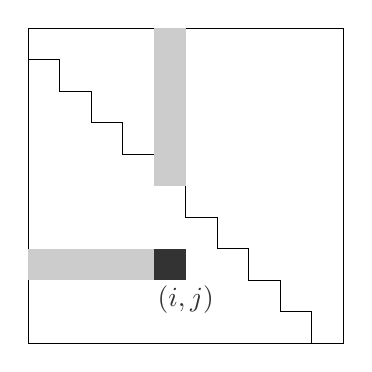
\begin{tikzpicture}[scale=0.4]
      \draw (0,0) rectangle ++ (10,10);
      \draw
      (0,9) --
      (1,9) --
      (1,8) --
      (2,8) --
      (2,7) --
      (3,7) --
      (3,6) --
      (4,6) --
      (4,5) --
      (5,5) --
      (5,4) --
      (6,4) --
      (6,3) --
      (7,3) --
      (7,2) --
      (8,2) --
      (8,1) --
      (9,1) --
      (9,0);
      \fill[black!20] (4,5) rectangle ++ (1,5);
      \fill[black!20] (0,2) rectangle ++ (4,1);
      \fill[black!80] (4,2) rectangle ++ (1,1) node[below=1em] {\((i,j)\)};
    \end{tikzpicture}
    \caption{Dependence for some \(l_{ij}\)}
  \end{subfigure}
  \begin{subfigure}{.4\linewidth}
    \centering
    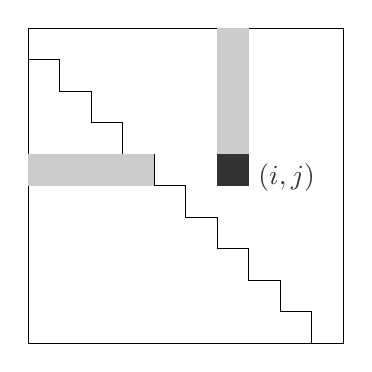
\begin{tikzpicture}[scale=0.4]
      \draw (0,0) rectangle ++ (10,10);
      \draw
      (0,9) --
      (1,9) --
      (1,8) --
      (2,8) --
      (2,7) --
      (3,7) --
      (3,6) --
      (4,6) --
      (4,5) --
      (5,5) --
      (5,4) --
      (6,4) --
      (6,3) --
      (7,3) --
      (7,2) --
      (8,2) --
      (8,1) --
      (9,1) --
      (9,0);
      \fill [black!20] (6,6) rectangle ++ (1,4);
      \fill [black!20] (0,5) rectangle ++ (4,1);
      \fill [black!80] (6,5) rectangle ++ (1,1) node[below right] {\((i,j)\)};
    \end{tikzpicture}
    \caption{Dependence for some \(u_{ij}\)}
  \end{subfigure}
  \caption[Dependence of ILU unknowns]{Formula for unknown at \((i,j)\) (dark
    square) depends on other unknowns left of \((i,j)\) in \(\matr{L}\) and
    above \((i,j)\) in \(\matr{U}\) (shaded regions).}
  \label{fig:dependence}
\end{figure}
